% Ubah judul dan label berikut sesuai dengan yang diinginkan.
\section{Penelitian dan Pembahasan}
\label{sec:PenelitianPembahasan}

Penelitian dilakukan dengan melakukan uji dan anaisa dari sistem yang telah dibuat berdasarkan langkah pada metodologi yang telah dilaksanakan. Pengujian ini dilakukan untuk menguji kemampuan sistem yang telah dibuat dalam menjawab permasalahan yang dijadikan acuan pada penelitian ini untuk mendapatkan hasil dari tujuan yang ingin didapat. Pembahasan pengujian yang dilakukan pada penelitian ini meliputi pengujian hasil training dan validation model, pengujian hasil testing model, pengujian hasil deteksi dan pengujian prediksi.

\subsection{Pengujian Hasil Training dan Validation Model}
\label{subsec:PengujianTrainingValidation}

Pengujian pembuatan model berdasarkan hasil training dan validation dengan menggunakan dataset dengan jumlah keseluruhan yaitu 1731 sampel data. Dengan jumlah sample training sebanyak 1385 dan sampel validation sebanyak 346. Setelah dilakukan proses training dan validation terhadap dataset yang telah ditentukan oleh sampel data, didapatkan hasil pengujian akurasi dengan tingkat akurasi training sebesar 0,951 dan tingkat akurasi validation sebesar 0,977. Kemudian didapatkan hasil pengujian loss pada training sebesar 0,127 dan loss pada validation sebesar 0,059. Hasil pengujian ditunjukkan pada grafik nilai akurasi dan loss pada proses training dan validation seperti pada Gambar \ref{fig:GrafikTrainingValidation}

\begin{figure} [ht]
  \centering
  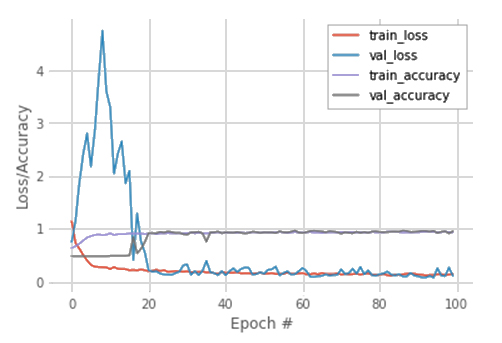
\includegraphics[width=0.4\textwidth]{gambar/hasil training dan validation w.jpg}
  \caption{Grafik Hasil Training dan Validation Model}
  \label{fig:GrafikTrainingValidation}
\end{figure}

\subsection{Pengujian Testing Model}
\label{subsec:PengujianTesting}

Pengujian dilanjutkan dengan melakukan \emph{testing} model dengan menggunakan dataset yang sudah dimiliki dengan jumlah keseluruhan yaitu 347 sampel data. Hasil pengujian \emph{testing} model didapatkan akurasi sebesar 95\% dengan hasil deteksi benar untuk kelas kanan sebanyak 170 sampel (96\%) dan kelas kiri sebanyak 161 sampel (95\%). Pengujian ditunjukkan dengan confusion matrix pada Gambar \ref{fig:HasilTesting} dan Tabel \ref{tab:ClassificationReport} merupakan classification report dari hasil pengujian yang telah dilakukan pada pengujian \emph{testing} model penelitian ini.

\begin{figure} [ht]
  \centering
  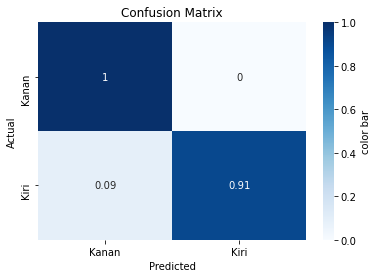
\includegraphics[width=0.4\textwidth]{gambar/cm normalized.png}
  \caption{\emph{Confusion Matrix} Hasil Pengujian Testing Model}
  \label{fig:HasilTesting}
\end{figure}

\begin{table} [ht]
  \caption{\emph{CLASSIFICATION REPORT} hasil pengujian \emph{TESTING} model}
  \label{tab:ClassificationReport}
  \centering
  \begin{tabular}{lllll}
    \toprule
     & Precision & Recall & F1-Score & Support  \\
    \midrule
    Kanan       & 0,91    & 1,00    & 0,96    & 170         \\
    Kiri        & 1,00    & 0,91    & 0,95    & 177           \\
    Accuracy    &         &         & 0,95    & 347            \\
    \bottomrule
  \end{tabular}
\end{table}

\subsection{Pengujian Hasil Deteksi}
\label{subsec:PengujianDeteksi}

Proses deteksi yang dilakukan dengan menggunakan model yang telah dibuat dilakukan pengujian dari hasil yang didapat dari hasil deteksi dengan perhitungan yang sebenarnya. Pengujian dilakukan dengan membuat data sebenarnya dengan melakukan perhitungan langkah dari akuisisi maupun data video yang digunakan dalam percobaan dan dibandingkan dengan hasil perhitungan langkah dari hasil deteksi. Tabel \ref{tab:PengujianDeteksi} menunjukkan hasil perhitungan data sebenarnya dengan data hasil deteksi terhadap langkah pada data video. Hasil yang didapat dengan melakukan pengujian hasil deteksi didapatkan hasil akurasi sebesar 99,36\% dengan hasil error sebesar 0,64\%.

\begin{table} [ht]
  \caption{Pengujian Hasil Deteksi}
  \label{tab:PengujianDeteksi}
  \centering
  \begin{tabular}{lll}
    \toprule
    Percobaan & Langkah & Deteksi Langkah  \\
    \midrule
    1   & 241   & 238    \\
    2   & 169   & 170    \\
    3   & 302   & 302    \\
    4   & 246   & 248    \\
    5   & 321   & 322    \\
    6   & 220   & 218    \\
    \bottomrule
  \end{tabular}
\end{table}


\subsection{Pengujian Prediksi}
\label{subsec:PengujianPrediksi}

Pengujian pada prediksi jumlah kalori yang terbakar dilakukan setelah melakukan pengujian pada model deteksi yang telah dilakukan. Prediksi dilakukan dengan dua metode, yaitu regresi linear dan perhitungan rumus. Dengan menggunakan dataset berupa citra video yang akan digunakan untuk melakukan prediksi kalori sebanyak 6 sampel video sehingga terdapat 6 percobaan yang dilakukan. Pada pengujian dengan regresi linear dengan melakukan proses deteksi dan menggunakan model regresi linear dalam melakukan proses prediksi kalori didapatkan beberapa data pendukung dalam hasil deteksi dan data dari hasil regresi prediksi kalori. Tabel \ref{tab:PengujianPrediksiRegresi} menunjukkan hasil deteksi dan hasil prediksi kalori dengan menggunakan regresi linear.

\begin{table} [ht]
  \caption{Pengujian Prediksi dengan Regresi Linear}
  \label{tab:PengujianPrediksiRegresi}
  \centering
  \begin{tabular}{lllll}
    \toprule
    Percobaan & Langkah & Jarak  &  Waktu & Kalori \\
    \midrule
    1   & 238   & 167,181    & 2:50    & 11,652  \\
    2   & 170   & 118,437    & 1:35    & 8,245   \\
    3   & 302   & 293,143    & 2:02    & 20,534  \\
    4   & 248   & 284,417    & 1:41    & 19,927  \\
    5   & 322   & 287,577    & 2:03    & 20,14   \\
    6   & 218   & 286,18     & 1:21    & 20,056  \\
    \bottomrule
  \end{tabular}
\end{table}

Pada pengujian dengan perhitungan rumus berdasarkan MET dilakukan dengan melalui proses deteksi dan melakukan perhitungan rumus menghasilkan beberapa data pendukung dalam perhitungan rumus dan hasil prediksi kalori yang didapat. Tabel \ref{tab:PengujianPrediksiPerhitungan} menunjukkan hasil deteksi dan hasil prediksi kalori dengan menggunakan perhitungan rumus.

\begin{table} [ht]
  \caption{Pengujian Prediksi dengan Perhitungan Rumus}
  \label{tab:PengujianPrediksiPerhitungan}
  \centering
  \begin{tabular}{lllll}
    \toprule
    Percobaan & Kecepatan & MET  &  Waktu & Kalori \\
    \midrule
    1   & 3,626   & 2,003    & 2:50    & 6,788   \\
    2   & 5,016   & 2,733    & 1:35    & 4.744   \\
    3   & 8,943   & 9,323    & 2:02    & 22.462  \\
    4   & 10,893  & 10,721   & 1:41    & 20.575  \\
    5   & 8,151   & 8,533    & 2:03    & 22.126  \\
    6   & 13,041  & 11,985   & 1:21    & 19.331  \\
    \bottomrule
  \end{tabular}
\end{table}

Hasil yang diperoleh melalui model yang telah dibuat untuk deteksi dan melakukan prediksi sesuai metode yang dilakukan didapatkan hasil akumulasi kalori dengan prediksi regresi sebesar 93,61\% dengan akumulasi error sebesar 6,39\%. Kemudian prediksi dengan perhitungan rumus didapatkan hasil akumulasi akurasi kalori sebesar 81,03\% dengan akumulasi error sebesar 18,97\%. Tabel \ref{tab:PengujianPrediksi} merupakan hasil perbandingan antara dataset percobaan dengan nilai kalori pembanding dataset dengan proses prediksi.

\begin{table} [ht]
  \caption{Pengujian Hasil Prediksi Kalori}
  \label{tab:PengujianPrediksi}
  \centering
  \begin{tabular}{lllll}
    \toprule
    Percobaan & Kecepatan & Kalori  &  Regresi & Perhitungan \\
    \midrule
    1   & 3     & 10    & 11,652    & 6,788   \\
    2   & 6     & 10    & 8,245     & 4,744   \\
    3   & 9     & 20    & 20,534    & 22,462   \\
    4   & 12    & 20    & 19,927    & 20,575   \\
    5   & 8     & 20    & 20,14     & 22,126   \\
    6   & 12    & 20    & 20,056    & 19,331   \\
    \bottomrule
  \end{tabular}
\end{table}
